\documentclass[a4paper, norsk, 12pt]{article}
\usepackage[T1]{fontenc}
\usepackage{fancyvrb}
%\documentclass{article} % was article, thought i'd try with report...
\usepackage{float}
%\usepackage{fullpage} % 1 inch margins
%\usepackage{harvard} % harvard reference style++
\usepackage[hidelinks]{hyperref} % do not remember entirely what this does
%%\usepackage{minted} % [LINUXONLY] list environment with code highlighting
\usepackage[utf8]{inputenc} %To get æøå
\usepackage[norsk]{babel} %Does it norway'ish
%\setcounter{chapter}{-1} %chapter numeration to start on 0
%\usepackage{titlesec} %To make chapter headings different
\usepackage[margin=2.5cm]{geometry}
%\usepackage{longtable} %Table that breakes pages
%\usepackage{tabularx} %Table that breakes lines
%\usepackage{ltablex} %Table that combines longtable and tubularx. (Use \begin{tabularx}
\usepackage{graphicx} %To insert image
\usepackage{parskip} %Removes indent and make space between the part sections, like \medskip.
\usepackage[labelformat=empty]{caption} %Removes "Figur 'nr'" in \caption on images.
%\usepackage{color, colortbl} %To use colors in tabulars


\newcommand{\tab}{\hspace*{2em}}

%Removes the indent:
%\setlength\parindent{0pt}

%Changing the paragraph title look:
\makeatletter
\renewcommand\paragraph{\@startsection{paragraph}{4}{\z@}%
  {-3.25ex\@plus -1ex \@minus -.2ex} %To get new line after title
  {1.5ex \@plus .2ex}%
  {\normalfont\large\bfseries}}
\makeatother

%\titleformat{\chapter}[hang]{\bf\huge}{\thechapter}{2pc}{} %To make chapters nice
\title{Oblig 1 \\ IMT3441 \\ Database- og applikasjonsdrift}
\author{Solveig Sørheim 090880 \\ Martin Kristian Mellum 100874}
\date{\today}


\begin{document}
\begin{figure}[h!]
 \centering
  
\includegraphics[width=0.5\textwidth]{Images/hig_logo.png}
 %\caption{Bare noko eg skribla på Paint..}
 \maketitle       % make title
\end{figure}
\pagebreak
%%\section{Abstract} % not sure if needed
%%This section is to be written when all else is done. 100-200 words summarizing.
\tableofcontents % make table of contents
\pagebreak	% and break the page, because pretty

\section{Ukesoppgaver Nr. 1 - 18. Januar}
\subsection{Oppgave 5}
\begin{itemize}
\item Vi installerte screen ganske greitt ved å følge retningslinjene i forelesingsfoilerne.
\item Startet en skreen ved å skrive screen -S “Navnet på screenen”
\item Gikk inn i en eksisterende screenen ved å skrive screen -r “Navn på screenen”
\item Bli med i en screen sammen en andre ved å skrive screen -x “Navn på screenen”
\item Går ut av screenen ved å presse Ctrl+a og Ctrl+d
\item Vi slettet en screen ved å først gå inn i screen sesjonen, deretter trykke control+a, og så shift+punktum, og deretter i kommandolinjen skrive quit.
\end{itemize}

\subsection{Oppgave 7}
\begin{figure}[h!]
 \centering
  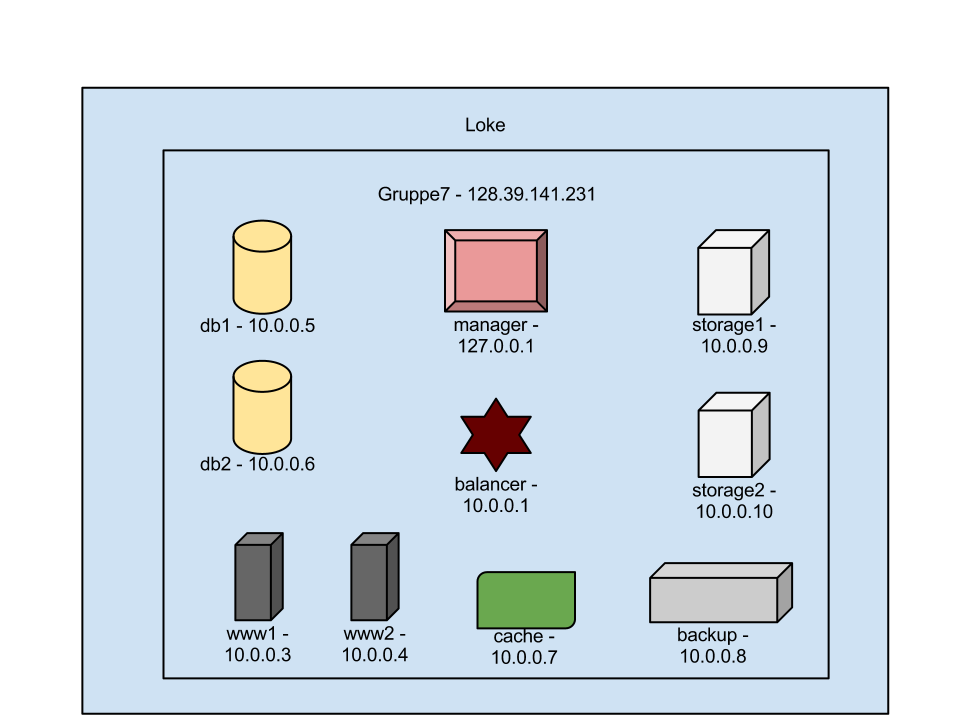
\includegraphics[width=1\textwidth]{Images/Gruppe7-IMT3441_Serverpark.png}
  \caption{Serverpark}
\end{figure}

\subsection{Oppgave 8}
\begin{description}
\item[10 \% Informasjonsintegritet - Backup \& Restore:]
 Systemadministrator må regelmessig ta backup av systemet, serverane og databasene. Dette kan gjøres automatisk, der systemadmin bare sjekker om backup vart gjort. Administratoren skal også ta større backuper ved andre tidspunkt. Dette tar ikke så lang tid. Å restore systemet skjer svært sjeldent.

\item[10 \% Adgangskontroll - Brukere \& Passord:]
Der kommer stadig nye brukere til systemet. Ettersom hvor mange brukere som kommer vil admin bruke variabelt med tid til dem. Men dette er en hurtig prosess, som ikke tar lang tid.

\item[35 \% Vedlikehold - Oppgradering \& Feilretting:]
Det viktigeste ansvaret til admin er vedlikehold, for å sørge for god vedlikehold vil minske risikoen for systemet. Der kommer stadig nye feil, og stadig må systemet oppgraderes. Derfor tar dette mest tid.

\item[25 \% Overvåking - Alarmer \& Ytelse over tid:]
Overvåkning er en veldig viktig del av jobben, og er måten man kan sjekke om alt annet fungerer slik det skal, men det tar tid og er en tidkrevende prossess å gå igjennom logger og system prosesser for å se at ting fortsetter å gå.

\item[10 \% Veiledning - Brukere \& Ny teknologi:]
Dette er en viktig del av jobben for at brukerene skal kunne bruke systemet, men det holder i stor grad å lage gode guider og FAQ’er, også slipper man mye manuell hjelping og spørsmål.

\item[10 \% Design - Infrastruktur:]
Design er en viktig jobb for å gjøre ting enkelt å bruke og forstå, men det gjøres gjerne en gang i starten, og i rykk og napp etterhvert som det må legges til ting, eller det gamle designet er utdatert, og er ikke noe som vanligvis endres å justeres hver dag.
\end{description}

\subsection{Oppgave 9}
Vi har fulgt forelesingsslidene når vi installerte munin. Da vi endret config-filen i manager så la vi inn de 9 andre servernavnene slik som eksempelet i forelesingsfoilene.
\begin{itemize}
\item Installert munin - done
\item Installert apache - done
\item Endret config filer - done
\end{itemize}

Installere noder og endret config:
\begin{itemize}
\item Storage1 - done
\item Storage2 - done
\item www1 - done
\item www2 - done
\item db1 - done
\item db2 - done
\item cache - done
\item manager - done
\item balancer -done
\item backup - done
\end{itemize}

\section{Ukesoppgaver Nr. 2 - 25. Januar}
\subsection{Oppgave 1}
Vi jobbet mye med å finne ut hva som var gale med å lage en nøkkelbasert innlogging fra manager til de andre maskinene. Vi prøvde mange kombinasjoner, forskjellige lagringsplasser, med og uten passord, forskjellege -t -i++, og andre kombinasjoner. Til slutt fann vi ut at problemet var at vi hadde lagret key-ene i en egen separat mappe, men at den skulle ligge under en spesifikk key-mappe(default). Da fikk vi laget en key i gruppe7 og sendt public keyen til de andre maskinene. Etterpå fann vi ut at det var root som skulle ha key, og ikkje gruppe7, so da måtte vi lage en ny key som root. Da måtte  vi overwrite keyen i gruppe7. Vi brukte disse kodene, og vi har ingen passord:\\
\begin{verbatim}
  ssh-keygen -t rsa
  eksempel: ssh-copy-id root@www1
\end{verbatim}
Det var denne nettsida som til slutt gav oss inspirasjon til svaret:\\
\begin{Verbatim}[samepage=true]
http://www.thegeekstuff.com/2008/11/3-steps-to-perform-ssh-login-without-password-using-ssh-keygen-ssh-copy-id/#more-268
\end{Verbatim}

En fordel med nøkkelbasert innlogging er at det gjør det mulig å logge seg inn noenlunde sikkert, uten å skrive inn passord. Dersom en skrev inn et passordet til nøkkelen, vil dette bekrefte at du er den personen som det er meningen skal bruke den private nøkkelen. Nøkkelbasert innlogging er sett på som mykje meir sikkert enn passordbasert innlogging, når en tenker på angrep fra et tredjepartsystem. Sjangsen for å knekke nøkkelen er veldig redusert i forhold til å knekke et vanlig dårlig passord.\\

Ulempene med nøkkelbasert innlogging er at om noen først kommer seg inn i systemet kan den enkelt bevege seg rundt mellom de forskjellige maskinene uten å måtte knekke et nytt passord for hver maskin.

<<<<<<< HEAD
\subsection{Oppgave 2}
Vi brukte kommandoen “uptime” og fekk dette resultatet:\\
16:00:33 up 40 days, 18:44, 32 users,  load average: 0.19, 0.14, 0.10\\
=======
\subsection*{Oppgave 2}
\begin{verbatim}
Vi brukte kommandoen “uptime” og fekk dette resultatet:
16:00:33 up 40 days, 18:44, 32 users,  load average: 0.19, 0.14, 0.10
\end{verbatim}
>>>>>>> Added unfinished part 2

Dersom vi bryter ned resultatet får vi:\\
\begin{enumerate}
\item 16:00:33
\item 40 days
\item 18:44
\item 32 users
\item load average: 0.19, 0.14, 0.10
\end{enumerate}

Punkt 1 er den nåværende tiden, dvs tidspunktet vi la inn kommandoen “uptime”\\
Punkt 2 er hvor lenge maskinen har vært oppe siden forrige start.\\
Punkt 3 er tidspunktet maskinen vart startet.\\
Punkt 4 er Antall brukere som er koblet til maskinen.\\
Punkt 5 er hvor mange prosesser som i gjennomsnitt er kjørt det siste minuttet, de siste fem minutter, og det siste kvarteret.\\

\begin{verbatim}[samepage=true]
Vi gjekk inn på .bashrc ved å bruke nano. Og der slet vi veldig med å få aliasen til å fungere. Det var variabelen $maskin som var problemet. Den ble ikke registrert. Så da prøvde vi enkelt-klaffer og dobbelt-klaffer innenfor og utenfor dollartegnet, der til slutt $”maskin” fungerte, med dobbelt-klaff innenfor dollartegnet. Deretter ville vi ha navnet til maskinen med i aliasen for bedre leselighet, så da la vi til en printf. For å gjøre linjene like lange tok vi å la inn “%-10s”.
\end{verbatim}

Koden så slik ut:
\begin{verbatim}
alias uptimeAll="for maskin in db1 db2 www1 www2 storage1 storage2 backup cache balancer manager; do printf "%-10s" $"maskin": ;  ssh $"maskin" uptime; done"
\end{verbatim}

Resultatet ser slik ut:\\
\begin{tabular}{lllll}
db1: & 20:42:36 up 40 days, & 23:27, & 2 users, & load average: 0.01, 0.06, 0.06\\
db2: & 20:42:36 up 40 days, & 23:27, & 2 users, & load average: 0.01, 0.05, 0.06\\
www1: & 20:42:37 up 40 days, & 23:26, & 4 users,& load average: 0.01, 0.06, 0.06\\
www2: & 20:42:37 up 40 days, & 23:26, & 2 users,& load average: 0.01, 0.07, 0.07\\
storage1: & 20:42:37 up 40 days, & 23:26, & 1 user, & load average: 0.01, 0.07, 0.07\\
storage2: & 20:42:37 up 40 days, & 23:26, & 1 user, & load average: 0.01, 0.07, 0.07\\
backup: & 20:42:37 up 40 days, & 23:27, & 1 user, & load average: 0.01, 0.04, 0.05\\
cache: & 20:42:37 up 40 days, & 23:27, & 2 users, & load average: 0.01, 0.06, 0.07\\
balancer: & 20:42:37 up 40 days, & 23:27, & 2 users, & load average: 0.00, 0.02, 0.05\\
manager: & 20:42:38 up 40 days, & 23:26, & 9 users, & load average: 0.10, 0.18, 0.21
\end{tabular}
\\

En slik kommando er nyttig for å kunne få en rask oversikt over hvor mange som bruker maskinene i øyeblikket, tilfellet en skulle ønske å gjøre noe service eller lignende og derfor starte maskinene på nytt. Eller for å sjekke hvor stor belastning det er på maskinene i tilfellet man ønsker å gjøre noe som krever mye ressurser. Vi kan også enkelt se om noen av maskinene er nede.

\subsection{Oppgave 9}
Vi valgte MemFree siden denne informasjonsbiten forteller oss hvor mye plass i minnet det er igjen i de forskjellige maskinene. \\

Koden såg slik ut:\\
for i in \{1..10\}; do printf "\%-10s" 10.0.0.\$i:; ssh 10.0.0.\$i cat /proc/meminfo | grep MemFree; done\\

Resultatet såg slik ut:\\
\begin{tabular}{lr}
10.0.0.1: MemFree: &         355512 kB\\
10.0.0.2: MemFree: &         992240 kB\\
10.0.0.3: MemFree: &        1085616 kB\\
10.0.0.4: MemFree: &        1186208 kB\\
10.0.0.5: MemFree: &        1215088 kB\\
10.0.0.6: MemFree: &        1214856 kB\\
10.0.0.7: MemFree: &        1215204 kB\\
10.0.0.8: MemFree: &        1217640 kB\\
10.0.0.9: MemFree: &        1218392 kB\\
10.0.0.10:MemFree: &        1218144 kB
\end{tabular}

\subsection{Oppgave 10}
Først prøvde vi å forstå dataane fra df -h, og prøvde å finne ut hvilken av linjene som representerte hvor mye plass det var ledig i serverene. Vi slet veldig med å finne ut hvordan grep fungerte på den måten at den skaffet bare dataane frå kolonne 4, dvs den kolonnen som het Avail. Vi brukte ofte manualen til grep, cut, awk og andre for å finne hint om hva vi kunne gjøre for å komme videre.\\

Flere kodesnutter feilet som f.eks:\\
\begin{verbatim}
df -h | cut -d\  -f1
df -h | grep "^.\{15\}"
df -h | egrep -v "Avail"
df -h | grep '^([^|]+\|){3}'
\end{verbatim}

Slik ser koden ut:\\
alias memfreeAll="\ for i in \{1..10\}; do printf "\%-10s" 10.0.0.\$"i":; ssh 10.0.0.\$"i"\ df -h | grep rootfs | tr -s ' ' | cut -d ' ' -f 4; done"\\

Slik ser resultatet ut:\\
10.0.0.1: 4.2G\\
10.0.0.2: 8.7G\\
10.0.0.3: 4.1G\\
10.0.0.4: 4.2G\\
10.0.0.5: 4.2G\\
10.0.0.6: 4.2G\\
10.0.0.7: 4.2G\\
10.0.0.8: 4.2G\\
10.0.0.9: 7.0G\\
10.0.0.10:7.0G

\section{Ukesoppgaver Nr. 3 - 01. Februar}
\subsection{Oppgave 1}
Vi installerte Apache og PHP på begge webserverene, ved å følge de retningslinjene i forelesingsfoileren. Vi passet på å være på webserverne da vi la inn apache og php.

\subsection{Oppgave 2}
Vi har testet ut om Apache fungerer ved å skrive fra manager:
\begin{itemize}
\item wget -q -O - http://10.0.0.3/
\item wget -q -O - http://10.0.0.4/
\end{itemize}
Vi lagde en index.php fil under mappen /var/www i begge webserverne, og testet php ved hjelp av denne koden fra manager:
\begin{itemize}
\item wget -q -O - http://10.0.0.3/index.php
\item wget -q -O - http://10.0.0.4/index.php
\end{itemize}

\subsection{Oppgave 3}
\begin{enumerate}
\item Vi følgte retningslinjene i forelesingsfoilerne.
\item Først lagde vi en fil i www1 med denne koden: nano /etc/apache2/conf.d/status
\item Deretter kopierte over informasjonen som skulle stå i fila, fra forelesingsfoileren.
\item Så la vi til en apacheplugin i munin og installerte perl. Tilslutt restartet vi munin-noden.
\item Deretter gjor vi det samme i www2.
\end{enumerate}

\subsection{Oppgave 4}
Vi har installert pound på balancer ved å bruke: apt-get install pound
Vi editerte så startup=1 i /etc/default/pound
Og i konfigurasjonsfila /etc/pound/pound.cfg (nb: .cfg) la vi inn

\begin{verbatim}
ListenHTTP
    Address 128.39.141.231
    Port    80

    ## allow PUT and DELETE also (by default only GET, POST and HEAD)?:\\
    xHTTP    0
    Service
        BackEnd
            Address 10.0.0.3
            Port    80
        End
        BackEnd
            Address 10.0.0.4
            Port    80
        End
    End
End
\end{verbatim}

Deretter lagde vi ein testfil: test.php i /var/www på både www1 og www2. Desse filane inneholder:
\begin{verbatim} 
<?php
echo "your IP: " . $_SERVER['REMOTE_ADDR'] . " ";
echo "served by: \"" . $_SERVER["SERVER_ADDR"] . "\"\n";
?>
\end{verbatim}

Vi prøvde å kjøre disse testfilene ved bruk av koden:
\begin{verbatim}
	wget -O - -q http://128.39.141.231/test.php 
\end{verbatim}
Men test.php gav ingen resultat. Den gav blankt svar.

Vi sendte epost til Kyrre Begnum og spurte om hva som var feil. Ved hjelp av svaret hans prøvde vi å teste direkte fra balancer om test.php virka på www1 og www2 ved hjelp av disse kodene:
\begin{verbatim}
wget -O - -q http://10.0.0.3/test.php
wget -O - -q http://10.0.0.4/test.php
\end{verbatim}

De ga svarene:
\begin{verbatim}
your IP: 10.0.0.1 served by: "10.0.0.3"
your IP: 10.0.0.1 served by: "10.0.0.4"
\end{verbatim}

Deretter sendte vi enda en epost til Kyrre Begnum, og fikk svar om at det var mest sannsynlig Pound i balancer som var feil. Etter anbefalinger fra Begnum prøvde vi:
\begin{verbatim}
ps aux | grep pound 
\end{verbatim}
og fikk resultatet:
\begin{verbatim}
gruppe7  23467  0.0  0.0   6288   596 pts/1    S+   10:30   0:00 grep pound
\end{verbatim}

Deretter prøvde vi igjen: wget -O - -q http://128.39.141.231/test.php for å sjekke kva resultat som vi fikk. Resultatet var det samme: ingen feilmeldinger, ingen resultat, og vi kom rett tilbake til kommandolinjen.

Vi sendte en epost tilbake til Begnum med resultatet. Begnum svarte raskt at det var pound som ikke hadde startet, og anbefalte oss å bruke koden “service pound start” for å starte pound.

Vi prøvde service pound start, men fikk error-beskjed om at cmd ikke kjente til kommandoen "service". Dermed letet vi litt på nettet og fant denne nettsiden:   https://help.ubuntu.com/community/Pound
der vi forsto at vi kanskje måtte vere root for å starte pound, og vi prøvde denne koden:
\begin{verbatim}
/etc/init.d/pound start
\end{verbatim}
Da skjedde det noe. Det virka som om pound startet.

Deretter prøvde vi: ps aux | grep pound, og fikk dette resultatet:
\begin{verbatim}
www-data 24416  0.0  0.1  34528   828 ?        Ss   10:47   0:00 /usr/sbin/pound
www-data 24418  0.0  0.2  68328  1848 ?        Sl   10:47   0:00 /usr/sbin/pound
root     24551  0.0  0.0   6288   596 pts/3    S+   10:47   0:00 grep pound
\end{verbatim}
Så prøvde vi i manager: wget -O - -q http://128.39.141.231/test.php, og fikk dette resultatet:
\begin{verbatim}
your IP: 10.0.0.1 served by: "10.0.0.4"
\end{verbatim}
Vi prøvde koden igjen og fikk: 
\begin{verbatim}
your IP: 10.0.0.1 served by: "10.0.0.3"
\end{verbatim} 
Disse to kommer annenhver gang fordi den balanserer belastninga på de to maskinene

\subsection{Oppgave 5}
Først installerte vi apache og rpaf modulet på manager slik det stod beskrevet i forelesningssliden. Så la vi til linjene fra sliden inn i apache sin http config fil, for deretter å restarte apache.

\subsection{Oppgave 6}
Vi prøvde å kode oppgaven først uten å bruke alias. Vi testet ut om hvilken kode vi måtte bruke for å slå av apache. Da vi fant det ut prøvde vi å teste ut om hvordan vi kunne skrive ut variabelnavn sammen med en tekst. Dette viste seg å ikke vere lett. Vi prøvde
\begin{verbatim}
for maskin in www1 www2; do printf “Stopper $maskin”
for maskin in www1 www2; do printf “Stopper” $”maskin”; done
\end{verbatim}
Men disse gav bare error. Vi prøvde så med echo, der dette gav ønsket resultat.
\begin{verbatim}
for maskin in www1 www2; do echo Stopper $maskin; done
\end{verbatim}
  Resultat:     
\begin{verbatim}
Stopper www1
Stopper www2
\end{verbatim}

Deretter prøvde vi å kombinere kodene og la de inn som alias. Dette førte til nye problem, for det å lage en tekst sammen med variabler som alias er ulikt dersom det ikke er alias. Vi måtte legge inn flere klaffer mm.

Dette er koden vi endte opp med først:
\begin{verbatim}
alias stopApacheWebservers="for maskin in www1 www2; do echo Stopper $"maskin"; ssh $"maskin" /etc/init.d/apache2 stop; done"
\end{verbatim}

Men så fann vi ut at det gav for liten leselighet så vi endte heller opp med denne koden:
\begin{verbatim}
alias stopApacheWS='for maskin in www1 www2; do printf "\nStopper apache paa %s:\n" $maskin; ssh $maskin /etc/init.d/apache2 stop; done'
\end{verbatim}

\subsection{Oppgave 7}
I utgangspunkt i koden i oppgave 6 ovanfor, lagde vi denne fungerende koden:
\begin{verbatim}
alias startApacheWS="for maskin in www1 www2; do echo Starter $"maskin"; ssh $"maskin" /etc/init.d/apache2 start; done"
\end{verbatim}

Men denne gav for liten leselighet, så vi endte heller opp med denne koden:
\begin{verbatim}
alias startApacheWS='for maskin in www1 www2; do printf "\nStarter apache paa %s:\n" $maskin; ssh $maskin /etc/init.d/apache2 start; done'
\end{verbatim}

\subsection{Oppgave 8}
I utgangspunkt i koden i oppgave 6 og 7 ovenfor, lagde vi denne fungerende koden:
\begin{verbatim}
alias restartApacheWS="for maskin in www1 www2; do echo Restarter $"maskin"; ssh $"maskin" /etc/init.d/apache2 restart; done"
\end{verbatim}

Men denne gav for liten leselighet, så vi endte heller opp med denne koden:
\begin{verbatim}
alias restartApacheWS='for maskin in www1 www2; do printf "\nRestarter apache paa %s:\n" $maskin; ssh $maskin /etc/init.d/apache2 restart; done'
\end{verbatim}

\subsection{Oppgave 9}
\subsubsection*{Oppgradering av database}
Databasen blir gjerne oppgradert i større eller mindre grad. Å legge til en ny tabell, en ny kolonne i en eksisterende tabell, oppsplitting av en eksisterende tabell til to eller flere nye tabeller, eller andre oppgraderinger krever nøye koordinasjon mellom databasedrift, applikasjonsdrift og SAN- og infrastruktur. Når databasen skal bli oppgradert, må gjerne databasen vere “nede”/ute av drift mens dette skjer. Dette betyr at f.eks. webserverne vert ute av drift også, og de må da gi tydelig bekjed til bruker om at oppgraderinger foregår, og når nettsiden er antatt å kome opp igjen. Det krev også koordinering med SAN- og infrastruktur siden der kan komme ny informasjon, og eksisterende informasjon må ikke gå tapt.

\subsubsection*{Backup}
Under en backupprosess er de andre nodene i driftsgruppen nødt til å koordineres, slik at de kan stoppe trafikken til den aktuelle noden som det tas backup av, slik at data ikke blir tapt. Enkelte webtjenester er nede er bestemt antall timer hver natt på grunn av backupprosesser.

\subsubsection*{Ny Release}
Når der kommer en ny release kreves dette koordinering mellom de ulike driftsgruppene. I en ny release vil applikasjonsdriftsgruppen gjøre endringene som trengs, og endringene vil foregå på serversiden. Da vil serverne vere “nede” i den perioden det tar for den nye releasen til å bli ferdig implementert. Ved ny release kommer det gjerne ny og annerledes informasjon som databasen må forholde seg til, og SAN- og infrastruktur må kanskje økes dersom det har for lite plass til forventningene til denne nye releasen.

\subsubsection*{Ny Release}
Ved utskifting av hardware må all trafikk gå rundt eller stoppes og krever derfor koordinering. Andre noder må derfor “vite” om dette, slik at de ikke prøver å ta i bruk en tjeneste eller maskin som ikke er oppe. Når utsikfitingen har skjedd, og all eventuell informasjon/data er flyttet over må alle noder i driftsgruppen på ny få en koordinering for at den akutuelle maskinen skal kunne tas i bruk.

\subsection{Oppgave 10}
Resultatet av denne kommandoen:
\begin{verbatim}
wget -O - -q http://www.vg.no | grep -i 'src="http' | wc -l
\end{verbatim}
forteller oss at kommandoen finner alle linjene i kildekoden som inneholder linker til andre nettsider.
Vi prøvde andre linker:
\begin{verbatim}
google.com      - 0 resultat
dagbladet.no    - 144 resultat
wikipedia.org   - 0 resultat
hig.no          - 1 resultat
finn.no         - 24 resultat
komplett.no     - 2 resultat
\end{verbatim}

Ettersom vi ser på resultatet virker det som det er en indikasjon på hvor mye reklame og annonser det finnes på en side. Resultatet viser kun linjene relatert til andre nettsider, så linker til egne nettsider vil ikke bli vist i resultatet. Derfor viser f.eks hig.no, google.com, wikipedia.org og komplett.no så få resultat. Vg.no og dagbladet.no har ekstremt mange annonser, og det kan vere grunnen til at de har de fleste resultatene.

Vi er usikker på om tallene vi får sier nøyaktig hvor mange annonser det finnes på siden, men man kan få en indikasjon på hvor mye reklame det er. Vi oppdaget at noen linker var tracking-baserte som bakgrunnskode basert på javascript. Vi antar at disse tracking-baserte resultatene kan hende var usynlige for den normale brukeren. I forhold til det vi først trudde, ved at kommandolinjen fann alle linjene på vg.no som inneholdt linker til andre nettsider, dvs poster, nyheter, mm., så er vi mer usikre nå. 

\section{Ukesoppgaver Nr. 4 - 08. Februar}
\subsection{Oppgave 1}
Vi fulgte how-to videoen fra fronter og støtte ikke borti noe problemet. Det eneste vi gjorde anerledes var å laste bookface-fila opp på dropbox og brukte wget til å laste den ned bookface derfra via en public link:\\
 wget http://dl.dropbox.com/u/10542464/bookface-1.0.tar.gz

%\clearpage
%\addcontentsline{toc}{section}{Referanser} %Add this section to content table
%\bibliographystyle{unsrt} % change for dcu, or something else entirely? unsrt is nice !- referanser
%\bibliography{Referanser}

%\addcontentsline{toc}{section}{Vedlegg} %Add this section to content table
%\section*{Vedlegg}

\end{document}